
\section{Expert Data Scientist User Study}
\label{sec:ds_baseline}

\iffalse
\begin{figure*}[!h]
    \centering
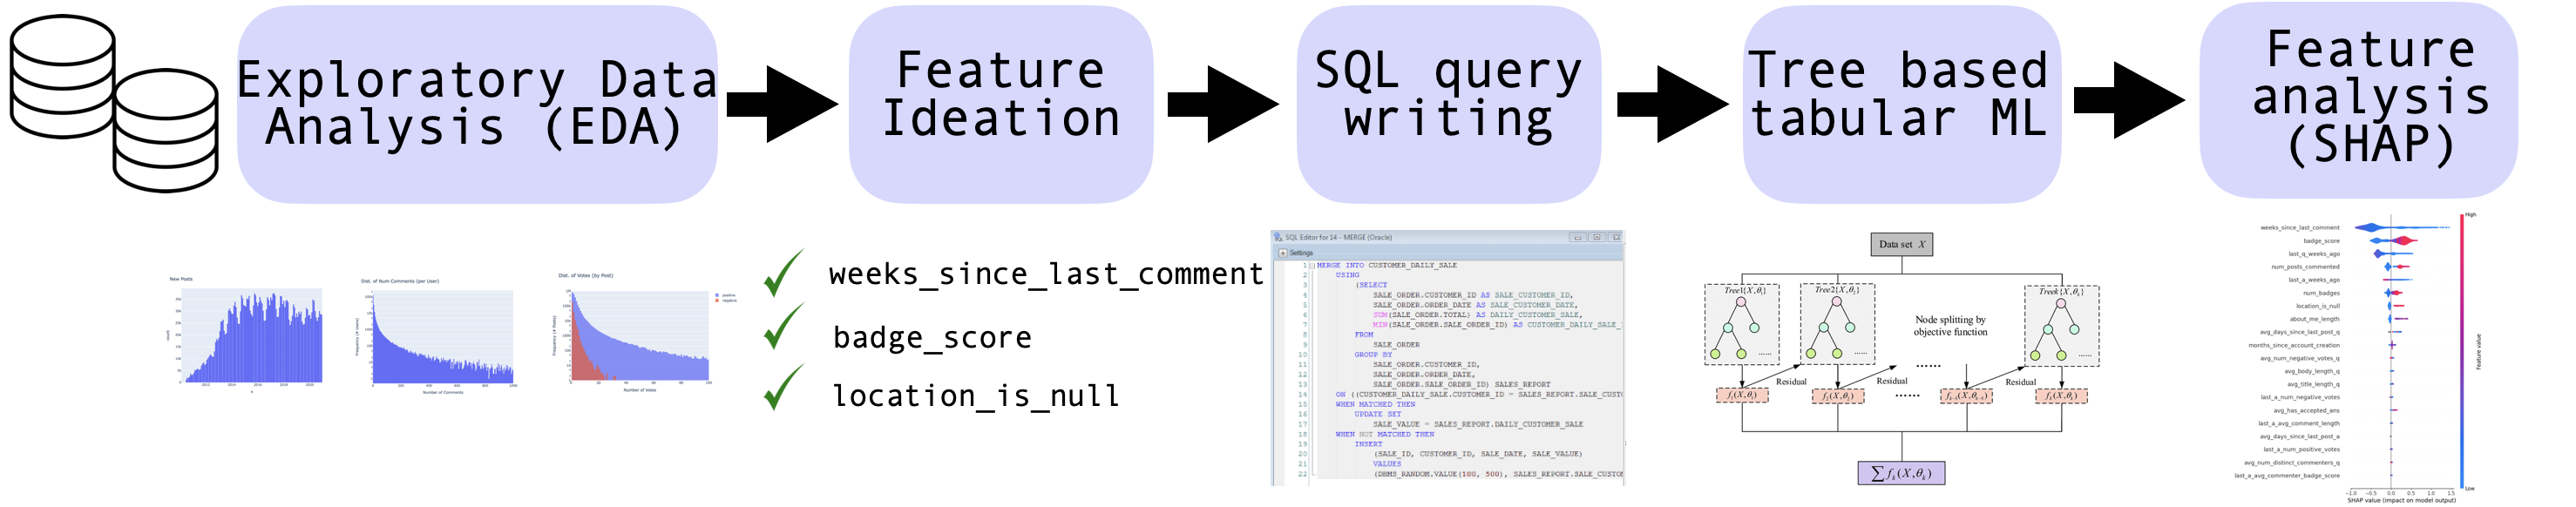
\includegraphics[width=\textwidth]{figs/user-study.png}
    \caption{\xhdr{\relbench user study} The traditional gold-standard model building pipeline for relational databases involves many steps and requires high-skilled manual work taking many hours and hundreds of lines of code, that must be redone every time a new task needs to be solved. .}
    \label{fig:rtb-fig-user-study}
\end{figure*}


\begin{figure}[htbp]
    \centering
    \subfigure{
        \includegraphics[width=0.9\textwidth]{figs/relbench_timings/0.png}
    }
    \\
    \vspace{-10pt}
    \subfigure{
        \includegraphics[width=0.9\textwidth]{figs/relbench_timings/1.png}
    }
    \\
    \vspace{-10pt}
    \subfigure{
        \includegraphics[width=0.9\textwidth]{figs/relbench_timings/2.png}
    }
    \vspace{-10pt}
    \caption{\xhdr{GNN vs Data Scientist} We compare: (i) predictive performance, (ii) hours of human work to build model, and (iii) number of lines of code written. We find GNNs enjoy strong predictive performance whilst requiring an order of magnitude less human work.\kexin{nice plot - for AUROC, maybe we can remove LightGBM? since this deviates our main message and it also raise question on why there is no lightgbm in the bottom two plots. another thing is for the upper panel, i think currently we could not see the performance difference, maybe consider starting the x-axis from 50 since random in AUROC is 50. also the legend should be outside of the figure. }} 
    \label{fig:ds main fif}
\end{figure}
\fi

%\wh{Any reason we have a separate section for data scientist? I would consider Tables 3--5 to be just ``sanity check'' without this expert data scientist baseline...}

To test RDL in the most challenging circumstances possible, we undertake a human trial wherein a data scientist solves each task by manually designing features and feeds them into tabular methods such at LightGBM or XGBoost~\citep{chen2016xgboost,ke2017lightgbm}. This represents the prior gold-standard for building predictive models on relational databases \citep{heaton2016empirical}, and the key point of comparison for RDL.

We structure our user study along the five main data science workflow steps:
%
\begin{enumerate}[leftmargin=0.6cm,itemsep=3pt, parsep=0pt]
    \item \textbf{Exploratory data analysis (EDA):} Explore the dataset and task to understand its characteristics, including what column features there are, and if there is any missing data.
    \item \textbf{Feature ideation:} Based on EDA and intuition from prior experiences, propose a set of entity-level features that the data scientist believes may contain predictive signal for the task.
    \item \textbf{Feature enginnering:} Using query languages such as SQL to compute the proposed features, and add them as extra columns to the target table of interest. 
    \item \textbf{Tabular ML:} Run tabular methods such as LightGBM or XGBoost on the table with extra features to produce a predictive model, and record the test performance.
    \item \textbf{Post-hoc analysis of feature importance (Optional):} Common tools include SHAP and LIME, which aim to explain the contribution of each input feature to the final performance. %\kexin{not sure if we need to mention this since we haven't discussed it?} \jr{Was planning to include in appendix}
\end{enumerate}

Consider for example the \handm dataset (schema in Appendix \ref{app:data}) and the task of predicting customer churn. Here the \tbl{customer} table only contains simple biographical information such as username and joining date. To capture more predictive information, additional features, such as  \emph{time since last purchase}, can be computed using the other tables, and added to the \tbl{customer} table. We give a detailed walk-through of the data scientist's work process for solving this specific task in Appendix \ref{app: user study}. We strongly encourage the interested reader to review this, as it highlights the significant amount of task-specific effort that this workflow necessitates.

\xhdr{Limitations of Manual Feature Engineering} This workflow suffers from several fundamental limitations. Most obviously, since features are hand designed they only capture part of the predictive signal in the database, useful signal is easily missed. Additionally, feature complexity is limited by human reasoning abilities, meaning that higher-order interactions between entities are often overlooked. Beyond predictive signal, the other crucial limitation of feature engineering is its extremely manual nature---every time a new model is built a data scientist has to repeat this process, requiring many hours of human labor, and significant quantities of new SQL code to design features \citep{zheng2018feature}. Our RDL models avoid these limitations (see Section \ref{subsec: user study results}).
%\wh{This paragraph feels repetitive of our intro}

\xhdr{Data Scientist} To conduct a thorough comparison to this process, we recruit a high-end data scientist with Stanford CS MSc degree, 4.0 GPA, and 5 years of experience of building machine learning models in the financial industry. This experience includes a significant amount of time building machine learning models in exactly above five steps, as well as broader data science expertise.

\xhdr{User Study Protocol} 
%EDA time is restricted to a maximum of 4 hours per dataset to limit complexity. Feature ideation is performed manually with pen and paper,  and is limited to 1 hour. In practice, the data scientist found that 1 hour was plenty of time to enumerate all promising features at that time. The time taken to write SQL code to generate the features is \emph{unconstrained} in order to eliminate code writing speed as a factor in the study. We do, however, record code writing time for our timing benchmarking. For tabular ML training, we provide a standardized LightGBM training script including comprehensive hyperparameter tuning. The data scientist needs only to feed the table full of engineered features into this training script, which returns test performance results. 
%

\begin{figure}[t]

\centering
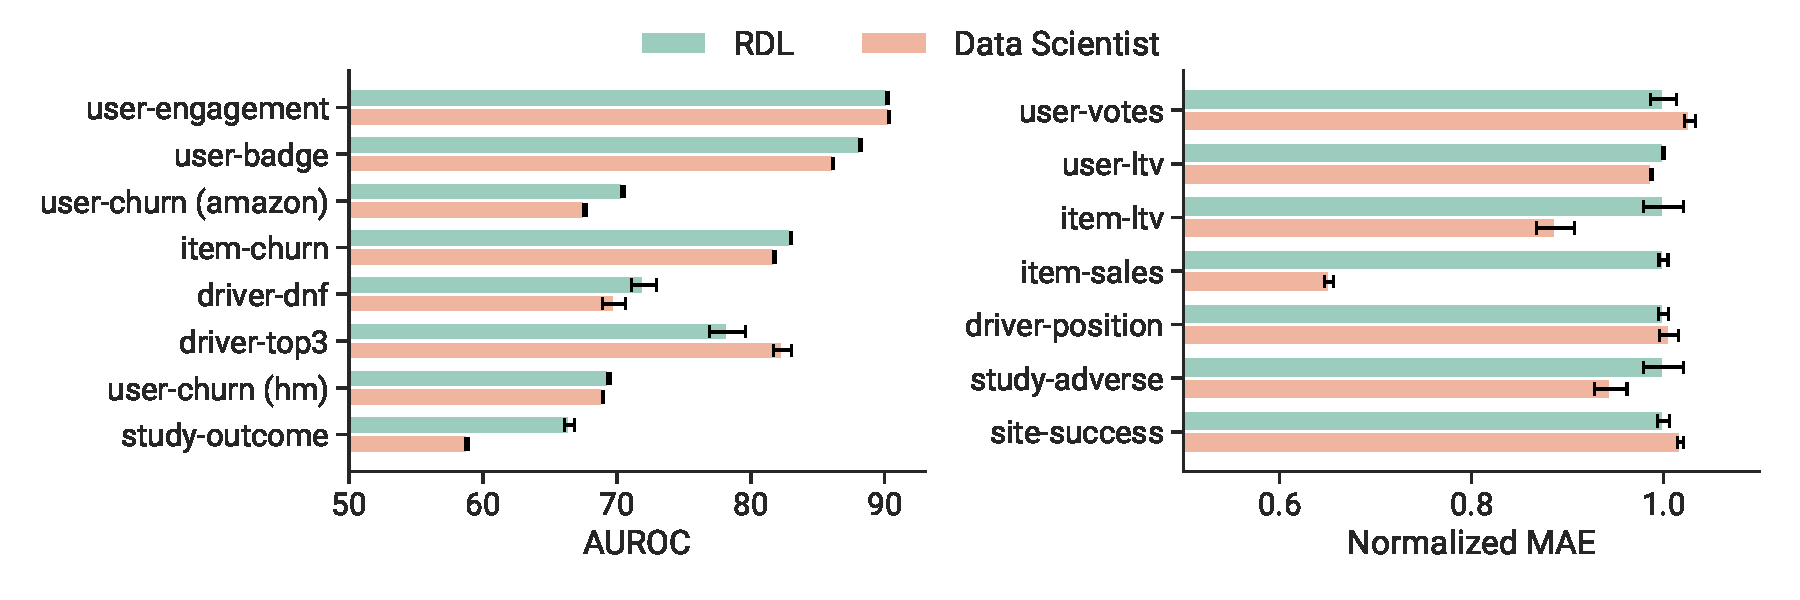
\includegraphics[width=\textwidth]{figs/combined_prediction.pdf}
\vspace{-20pt}
\caption{\textbf{RDL vs. Data Scientist.} Relational Deep Learning matches or outperforms the data scientist in 11 of 15 tasks. Left shows entity classification AUROC, right shows entity regression, reporting MAE normalized so that the RDL MAE is always 1.
}
\vspace{-5pt}
\label{fig:ds main fig}
\end{figure}

Because of the open-ended nature of feature engineering and model development, we follow a specific protocol for the user study in order to standardize the amount of effort dedicated to each dataset and task. Tracking the 5 steps outlined above, we impose the following rules:

\begin{enumerate}
\item \textbf{EDA:} The time allotted for data exploration is capped at 4 hours. This threshold was chosen to give the data scientist enough time to familiarize themselves with the schema, visualize key relationships and distributions, and take stock of any outliers in the dataset, while providing a reasonable limit to the effort applied.
\item \textbf{Feature ideation:} Feature ideation is performed manually with pen and paper, and is limited to 1 hour. In practice, the data scientist found that 1 hour was plenty of time to enumerate all promising features at that time, especially since many ideas naturally arise during the EDA process already.
\item \textbf{Feature engineering:} The features described during the ideation phase are then computed using SQL queries. The time taken to write SQL code to generate the features is unconstrained in order to eliminate code writing speed as a factor in the study. We do, however, record code writing time for our timing benchmarking. This stage presented the most variability in terms of time commitment, partly because it is unconstrained, but mostly because the implementation complexity of the features itself is highly variable.
\item \textbf{Tabular ML:} For tabular ML training, we provide a standardized LightGBM training script including comprehensive hyperparameter tuning. The data scientist needs only to feed the table full of engineered features into this training script, which returns test performance results. However, there is some non-trivial amount of work required to transform the output of the SQL queries from the previous section into the Python objects (arrays) required for training LightGBM. Again, the time taken for this additional pre-preocessing is recorded.
\item \textbf{Post-hoc analysis of feature importance:} Finally, after successfully training a model, an evaluation of model predictions and feature importance is carried out. This mostly serves as a general sanity check and an interesting corollary of the data scientist’s work that provides task-specific insights (see Appendix \ref{app: user study}). In practice, this took no more than a few minutes per task and this time was not counted toward the total time commitment.
\end{enumerate}


\xhdr{Reproducibility}  All of the data scientist's workings are released\footnote{See \userstudy.} to ensure reproducibility and demonstrate the significant lengths gone through to build as accurate models as possible. In Appendix \ref{app: user study} we walk through a complete example for a single dataset and task, showing the data-centric insights it yields. An important by-product is a close analysis of which features contribute to model performance, which we believe will help inspire future well-motivated RDL research directions. 



\begin{figure}[t]

\centering
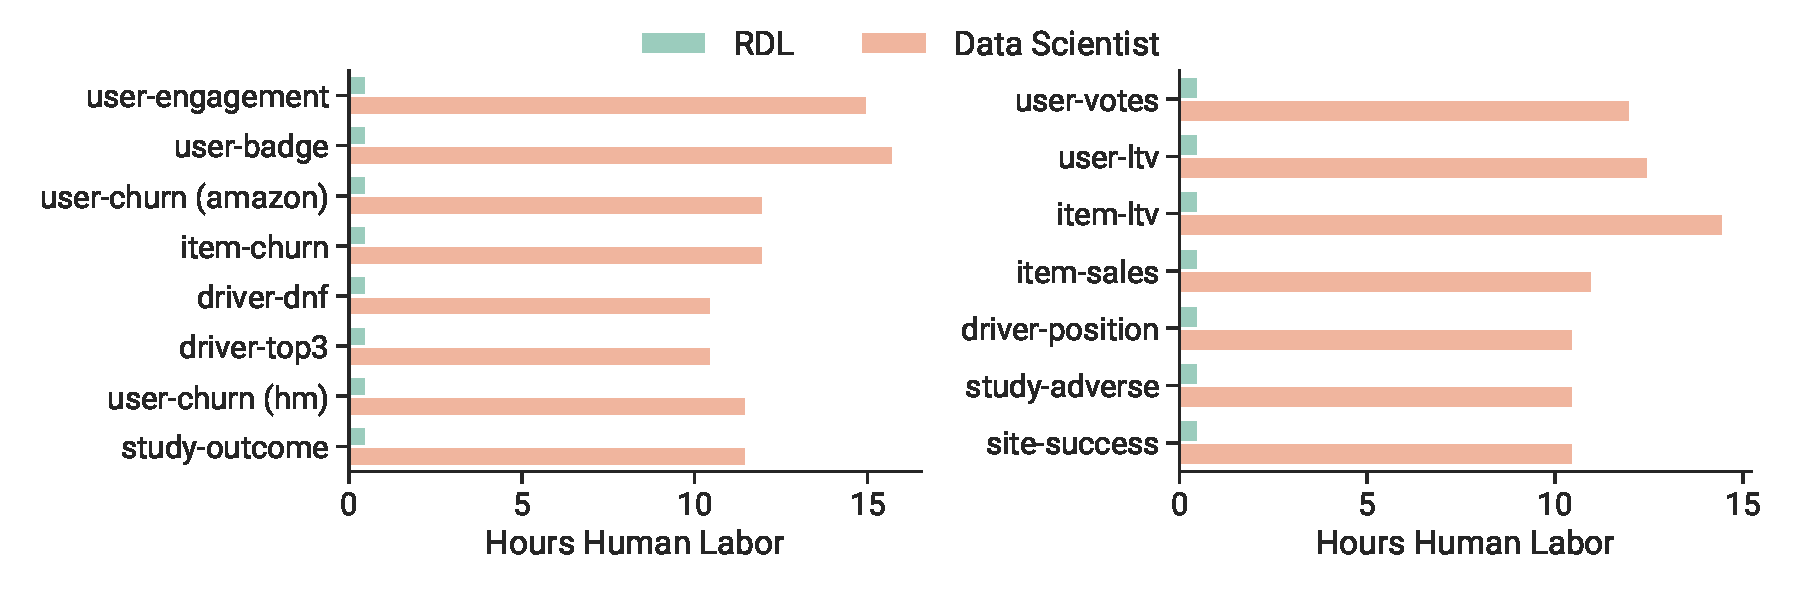
\includegraphics[width=\textwidth]{figs/combined_hours.pdf}
\vspace{-20pt}
\caption{\textbf{RDL vs. Data Scientist.} Relational Deep Learning reduces the hours of human work required to solve a new task by 96\% on average (from 12.3 to 0.5 hours). Left shows node-level classification, right shows node-level regression.
}
\vspace{-5pt}
\label{fig:ds main fig hours}
\end{figure}



\subsection{Results}\label{subsec: user study results}

As well as (i) raw predictive power, we compare the data scientist to our RDL models in terms of (ii) hours of human  work, and (iii) number of new lines of code required to solve each task. We measure the \emph{marginal} effort, meaning that we do not include code infrastructure that is reused across tasks, including for example data loading logic and training scripts for RDL or LightGBM models. 

\xhdr{Summary} Figures \ref{fig:ds main fig}, \ref{fig:ds main fig hours}, and \ref{fig:ds main fig lines} show that RDL learns highly predictive models, outperforming the data scientist in 11 of 15 tasks, whilst reducing hours worked by $96\%$ on average, and lines of code by $94\%$ on average. On average, it took the data scientist 12.3 hours to solve each task using traditional feature engineering. By contrast it takes roughly 30 minutes to solve a task with RDL.
% \jure{At the same time we also observe that RLD models are X\% more accurate on the average (X\% for entity classification, Y\% for entity regression, Z\% for link prediction).} \alejandro{Provisionally: X = 0.1\% and Y = -10.7\% and there is no Z (no user-study on link pred). Doesn't align with the message. IDK if we still want to include.}

This observation is \emph{the} central value proposition of relational deep learning, pointing the way to unlocking new levels of predictive power, and potentially a new economic model for solving predictive tasks on relational databases. Replacing hand-crafted solutions with end-to-end learnable models has been a key takeaway from the last 15 years of AI research. It is therefore remarkable how little impact deep learning has had on ML on relational databases, one of the most widespread applied ML use cases. To the best of our knowledge, RDL represents the first proposal for a deep learning approach for relational databases that has demonstrated efficacy compared with established data science workflows. 

We highlight that all \relbench tasks were solved with a single set of default hyperparameters (with 2 exceptions requiring small modifications to learning rate, number of epochs, and GNN aggregation function). This demonstrates the robustness of RDL, and that the performance of RDL in Figure \ref{fig:ds main fig} is not due to extensive hyperparamter search. Indeed, the single set of RDL hyperparameters is compared to a carefully tuned LightGBM, which was allowed to search over 10 sets of hyperparameters.

\xhdr{Predictive Power} Results shown in Figures \ref{fig:ds main fig}. Whilst  outperforming the data scientist in 11 of 15 tasks, we note that RDL best outperforms the data scientist on classification tasks, struggling more on regression. Indeed it was necessary for us to apply a ``boosting'' to the RDL model to improve performance (see Appendix \ref{app: user study} for details). Even with boosting, the data scientist model outperforms RDL in several cases. One cause we identify is that the MLP output head of the GNN is poorly suited to regression tasks (see Appendix \ref{app: user study} for our analysis). This suggests an opportunity for improved output heads for regression tasks. We stress that our RDL implementation is an \emph{initial} demonstration. We believe there is significant scope for new research leading to large improvements in performance. In particular, ideas from graph ML, deep tabular ML, and time-series modeling are well suited to advance RDL.

\begin{figure}[t]

\centering
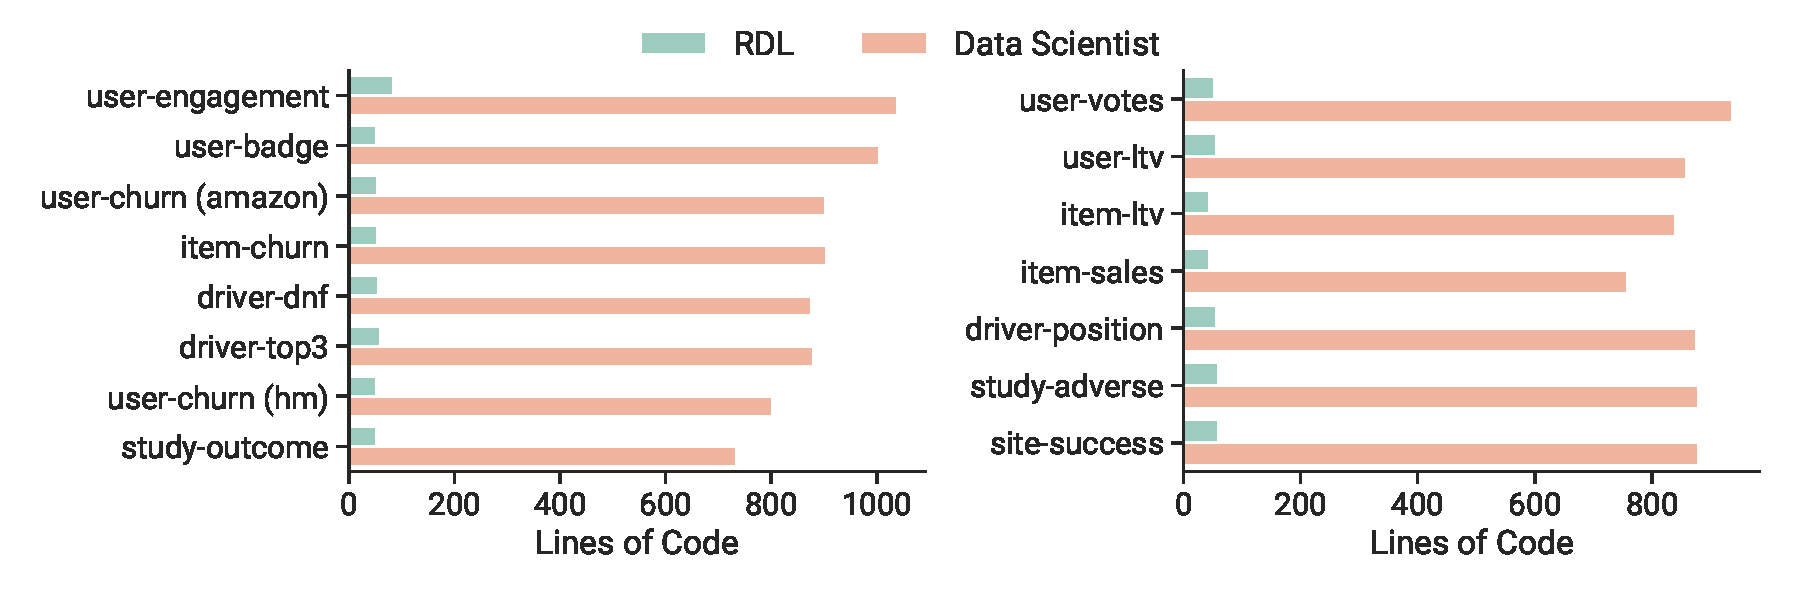
\includegraphics[width=\textwidth]{figs/combined_lines.pdf}
\vspace{-20pt}
\caption{\textbf{RDL vs. Data Scientist.} Relational Deep Learning reduces the new lines of code needed to solve a new task by 94\%. Left shows entity classification, right shows entity regression.
}
\vspace{-5pt}
\label{fig:ds main fig lines}
\end{figure}
\xhdr{Human Work} Results shown in Figure \ref{fig:ds main fig hours}. In our user study RDL required 96\% less hours work to solve a new task, compared to the data scientist work flow. The RDL solutions always took less than an hour to write, whilst the data scientist took $12$ hours on average, with a standard deviation of $1.6$ hours. We emphasize that this measures \emph{marginal} effort, i.e., it does not include reusable code that can be amortized over many tasks. RDL compares favorably to data scientist because a large majority of RDL code is reusable for new tasks (a GNN architecture and training loop needs only to be defined once) whereas a large portion of the data scientist's code is task specific and must be re-done afresh for every new task that needs to be solved. 

\xhdr{Lines of Code} Results shown in Figure \ref{fig:ds main fig lines}. For the RDL model, the only new addition needed to solve a new task is the code describing how to compute the training supervision for the RDL, which is stored in the training table. This requires a similar number of lines of code for each task, with 56 lines of code on average, with standard deviation $8.8$, with the data scientist requiring with $878 \pm 77$. The minimum lines of code required by RDL is 44, compared to 734 for the data scientist, and maximum is 84 compared to 1039 for the data scientist. Examples of the RDL code required to solve \amazon tasks can be viewed \href{https://github.com/snap-stanford/relbench/blob/main/relbench/tasks/amazon.py#L19}{here}. For the data scientist pipeline, we record the number of lines of code for EDA and SQL files, and the manipulations needed to format data to be fed into the pre-prepared LightGBM script. 